\documentclass[border=10pt,tikz]{standalone}
\usepackage[T1]{fontenc}
\usepackage{helvet}
\renewcommand{\familydefault}{\sfdefault}
\usepackage{tikz}
\usetikzlibrary{arrows.meta, positioning, shapes.geometric, backgrounds, fit, calc}

% ---- Professional engineering palette ----
\definecolor{camcol}{RGB}{31,56,100}      % deep navy
\definecolor{camfill}{RGB}{232,237,245}
\definecolor{lidcol}{RGB}{164,74,32}      % burnt sienna
\definecolor{lidfill}{RGB}{249,234,224}
\definecolor{fusecol}{RGB}{46,94,58}      % forest green
\definecolor{fusefill}{RGB}{230,240,232}
\definecolor{sensecol}{RGB}{70,70,70}     % charcoal
\definecolor{sensefill}{RGB}{240,240,240}
\definecolor{linecol}{RGB}{55,65,80}      % near-black slate

\begin{document}
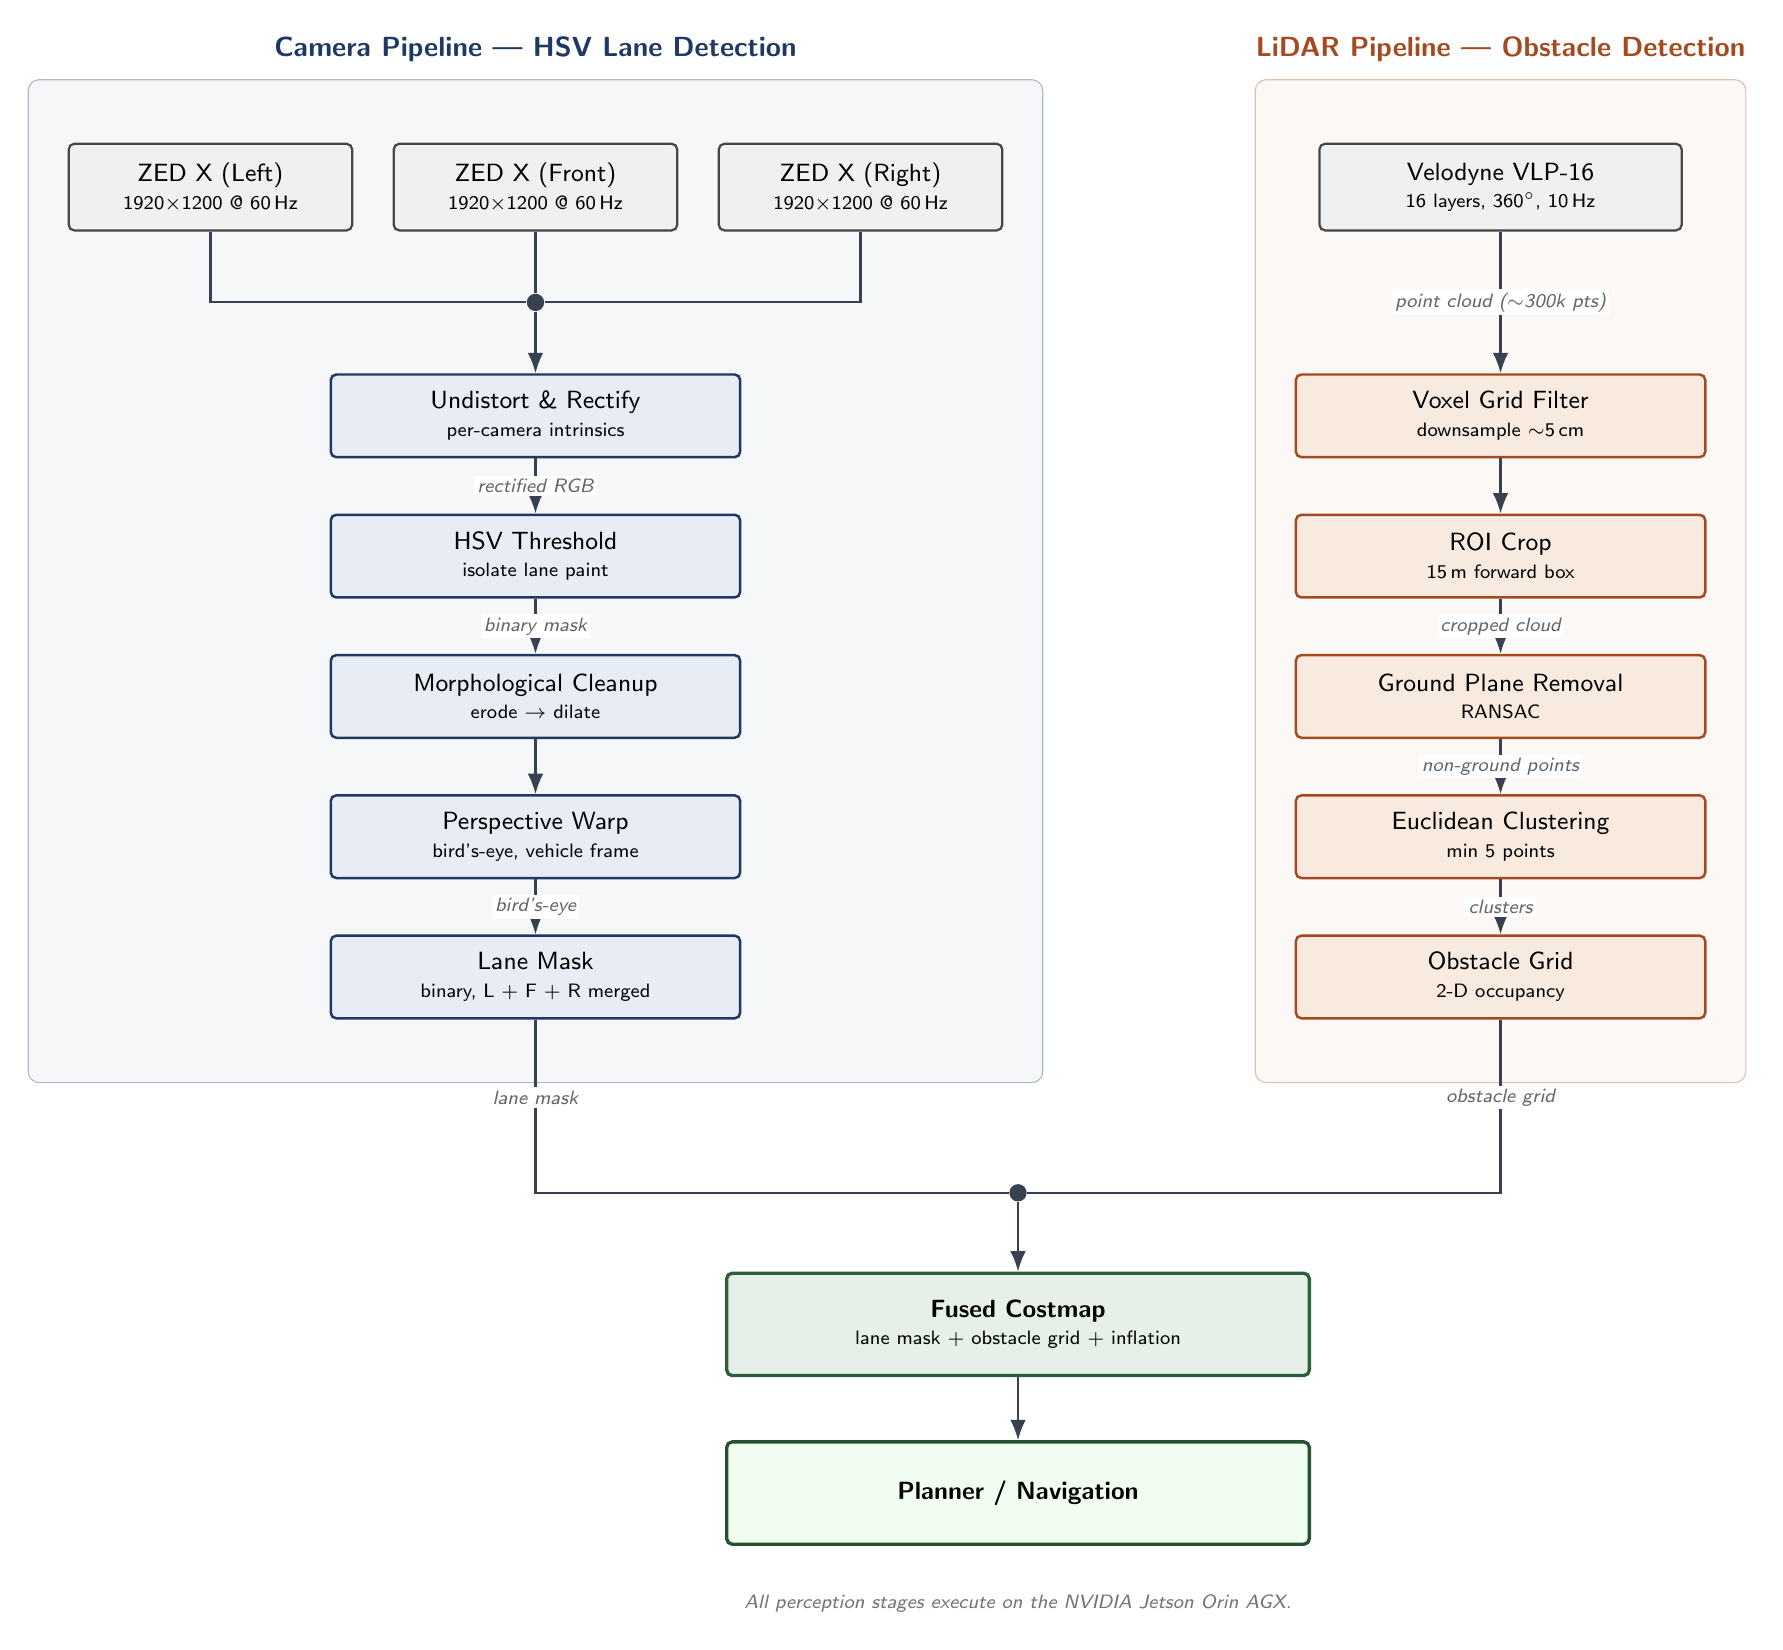
\begin{tikzpicture}[
    font=\sffamily\small,
    >={Latex[length=2.6mm, width=2mm]},
    node distance=7mm,
    block/.style={
        draw, line width=0.9pt, rounded corners=2pt,
        minimum width=52mm, minimum height=10.5mm,
        align=center, inner sep=1.5mm,
    },
    cam/.style={block, draw=camcol, fill=camfill},
    lid/.style={block, draw=lidcol, fill=lidfill},
    fuse/.style={block, draw=fusecol, fill=fusefill, line width=1.2pt,
                 minimum width=74mm, minimum height=13mm,
                 font=\sffamily\bfseries\small},
    sense/.style={block, draw=sensecol, fill=sensefill,
                  minimum width=36mm, minimum height=11mm,
                  line width=0.8pt},
    % clean arrow primitives
    arr/.style={->, line width=0.8pt, draw=linecol},
    line/.style={-,  line width=0.8pt, draw=linecol},
    junction/.style={circle, fill=linecol, inner sep=0pt, minimum size=2.2mm},
    edgelbl/.style={font=\scriptsize\itshape, text=black!60,
                    fill=white, inner sep=1.2pt},
]

% =====================================================================
% Camera inputs: 3 ZED X (Left / Front / Right)
% =====================================================================
\node[sense, minimum width=36mm] (zedl)
    {ZED X (Left)\\[-1pt]\scriptsize 1920$\times$1200 @ 60\,Hz};
\node[sense, right=5mm of zedl, minimum width=36mm] (zedf)
    {ZED X (Front)\\[-1pt]\scriptsize 1920$\times$1200 @ 60\,Hz};
\node[sense, right=5mm of zedf, minimum width=36mm] (zedr)
    {ZED X (Right)\\[-1pt]\scriptsize 1920$\times$1200 @ 60\,Hz};

% =====================================================================
% Camera processing column
% =====================================================================
\node[cam, below=18mm of zedf] (rect)
    {Undistort \& Rectify\\[-1pt]\scriptsize per-camera intrinsics};
\node[cam, below=of rect] (hsv)
    {HSV Threshold\\[-1pt]\scriptsize isolate lane paint};
\node[cam, below=of hsv] (morph)
    {Morphological Cleanup\\[-1pt]\scriptsize erode $\to$ dilate};
\node[cam, below=of morph] (warp)
    {Perspective Warp\\[-1pt]\scriptsize bird's-eye, vehicle frame};
\node[cam, below=of warp] (lanemask)
    {Lane Mask\\[-1pt]\scriptsize binary, L $+$ F $+$ R merged};

% =====================================================================
% LiDAR input + processing column
% =====================================================================
\node[sense, right=40mm of zedr, minimum width=46mm] (vlp)
    {Velodyne VLP-16\\[-1pt]\scriptsize 16 layers, 360$^\circ$, 10\,Hz};
\node[lid, below=18mm of vlp] (voxel)
    {Voxel Grid Filter\\[-1pt]\scriptsize downsample $\sim$5\,cm};
\node[lid, below=of voxel] (roi)
    {ROI Crop\\[-1pt]\scriptsize 15\,m forward box};
\node[lid, below=of roi] (ground)
    {Ground Plane Removal\\[-1pt]\scriptsize RANSAC};
\node[lid, below=of ground] (cluster)
    {Euclidean Clustering\\[-1pt]\scriptsize min 5 points};
\node[lid, below=of cluster] (obst)
    {Obstacle Grid\\[-1pt]\scriptsize 2-D occupancy};

% =====================================================================
% Fusion output
% =====================================================================
\coordinate (mid) at ($(lanemask.south)!0.5!(obst.south)$);
\node[fuse, below=32mm of mid] (costmap)
    {Fused Costmap\\[-1pt]\mdseries\scriptsize lane mask $+$ obstacle grid $+$ inflation};
\node[fuse, below=8mm of costmap,
      draw=fusecol!85!black, fill=fusefill!70!green!15,
      line width=1.2pt] (planner)
    {Planner / Navigation};

% =====================================================================
% Camera fan-in (3 ZED X -> Rectify) with junction dot
% =====================================================================
\node[junction] (camfan) at ($(zedf.south) + (0,-9mm)$) {};
\draw[line] (zedl.south) |- (camfan);
\draw[line] (zedf.south) -- (camfan);
\draw[line] (zedr.south) |- (camfan);
\draw[arr]  (camfan)     -- (rect.north);

% =====================================================================
% Camera stage arrows
% =====================================================================
\draw[arr] (rect)  -- node[edgelbl]{rectified RGB}  (hsv);
\draw[arr] (hsv)   -- node[edgelbl]{binary mask}    (morph);
\draw[arr] (morph) -- (warp);
\draw[arr] (warp)  -- node[edgelbl]{bird's-eye}     (lanemask);

% =====================================================================
% LiDAR stage arrows
% =====================================================================
\draw[arr] (vlp)     -- node[edgelbl]{point cloud ($\sim$300k pts)} (voxel);
\draw[arr] (voxel)   -- (roi);
\draw[arr] (roi)     -- node[edgelbl]{cropped cloud}     (ground);
\draw[arr] (ground)  -- node[edgelbl]{non-ground points} (cluster);
\draw[arr] (cluster) -- node[edgelbl]{clusters}          (obst);

% =====================================================================
% Two-into-one merge into Fused Costmap with junction dot
% =====================================================================
\node[junction] (fusejoin) at ($(costmap.north) + (0,10mm)$) {};
\draw[line] (lanemask.south) |- (fusejoin);
\draw[line] (obst.south)     |- (fusejoin);
\draw[arr]  (fusejoin)       -- (costmap.north);

% Label the two merging data streams on their vertical segments
\node[edgelbl] at ($(lanemask.south)!0.45!(fusejoin -| lanemask)$) {lane mask};
\node[edgelbl] at ($(obst.south)    !0.45!(fusejoin -| obst)$)     {obstacle grid};

% Costmap -> Planner
\draw[arr] (costmap) -- (planner);

% =====================================================================
% Swimlane backgrounds + titles
% =====================================================================
\begin{pgfonlayer}{background}
  \node[draw=camcol!35, rounded corners=4pt, fill=camcol!4,
        fit=(zedl)(zedr)(lanemask), inner sep=5mm, inner ysep=8mm,
        label={[text=camcol, font=\sffamily\bfseries, yshift=1mm]above:%
               Camera Pipeline \textemdash{} HSV Lane Detection}] {};
  \node[draw=lidcol!35, rounded corners=4pt, fill=lidcol!4,
        fit=(vlp)(obst), inner sep=5mm, inner ysep=8mm,
        label={[text=lidcol, font=\sffamily\bfseries, yshift=1mm]above:%
               LiDAR Pipeline \textemdash{} Obstacle Detection}] {};
\end{pgfonlayer}

% =====================================================================
% Compute-platform footer
% =====================================================================
\node[font=\scriptsize\itshape, text=black!55, below=5mm of planner]
    (footer) {All perception stages execute on the NVIDIA Jetson Orin AGX.};

\end{tikzpicture}
\end{document}
